% !TeX root = RJwrapper.tex
\title{Species Distribution Modeling using Spatial Point Processes: a Case Study of Sloth Occurrence in Costa Rica}
\author{by Paula Moraga}

\maketitle

\abstract{
Species distribution models are widely used in ecology for conservation management of species and their environments.%
This paper demonstrates how to fit a log-Gaussian Cox process model to predict the intensity of sloth occurrence in Costa Rica, and assess the effect of climatic factors on spatial patterns using the \pkg{R-INLA} package.
Species occurrence data are retrieved using \pkg{spocc}, and spatial climatic variables are obtained with \pkg{raster}.%
Spatial data and results are manipulated and visualized by means of several packages such as \pkg{raster} and \pkg{tmap}.%
This paper provides an accessible illustration of spatial point process modeling that can be used to analyze data that arise in a wide range of fields including ecology, epidemiology and the environment.}


  
\section{Introduction}

Species distribution models are widely used in ecology to predict and understand spatial patterns, assess the influence of climatic and environmental factors on species occurrence, and identify rare and endangered species.
These models are crucial for the development of appropriate strategies that help protect species and the environments where they live.
In this paper, we demonstrate how to formulate spatial point processes for species distribution modeling and how to fit them with the \pkg{R-INLA} package \citep{rueetal09} (\url{http://www.r-inla.org/}).

Point processes are stochastic models that describe locations of events of interest and possibly some additional information such as marks that inform about different types of events \citep{diggle13, moragaandmontes11}.
These models can be used to identify patterns in the distribution of the observed locations, estimate the intensity of events (i.e., mean number of events per unit area), and learn about the correlation between the locations and spatial covariates.
The simplest theoretical point process model is the homogeneous Poisson process. This process satisfies two conditions.
First, the number of events in any region $A$ follows a Poisson distribution with mean $\lambda |A|$, where $\lambda$ is a constant value denoting the intensity and $|A|$ is the area of region $A$. And second, the number of events in disjoint regions are independent.
Thus, if a point pattern arises as a realization of an homogeneous Poisson process, an event is equally likely to occur at any location within the study region, regardless of the locations of other events.


In many situations, the homogeneous Poisson process is too restrictive.
A more interesting point process model is the log-Gaussian Cox process which is typically used to model phenomena that are environmentally driven
\citep{diggleetal13}.
A log-Gaussian Cox process is a Poisson process with a varying intensity which is itself a stochastic process of the form $\Lambda(s) = exp(Z(s))$ where $Z = \{Z(s): s \in \mathbb{R}^2\}$ is a Gaussian process.
Then, conditional on $\Lambda(s)$, the point process is a Poisson process with intensity $\Lambda(s)$.
This implies that the number of events in any region $A$ is Poisson distributed with mean
$\int_A \Lambda(s)ds$, and the locations of events are an independent random sample from the distribution on $A$ with probability density proportional to $\Lambda(s)$.
The log-Gaussian Cox process model can also be easily extended to include spatial explanatory variables providing a flexible approach for describing and predicting a wide range of spatial phenomena.


In this paper, we formulate and fit a log-Gaussian Cox process model for sloth occurrence data in Costa Rica that incorporates spatial covariates that can influence the occurrence of sloths, as well as random effects to model unexplained variability.
The model allows to estimate the intensity of the process that generates the data, understand the overall spatial distribution, and assess factors that can affect spatial patterns.
This information can be used by decision-makers to develop and implement conservation management strategies.


The rest of the paper is organized as follows.
First, we show how to retrieve sloth occurrence data using the \CRANpkg{spocc} package \citep{Rspocc} and spatial climatic variables using the \CRANpkg{raster} package \citep{Rraster}.
Then, we detail how to formulate the log-Gaussian Cox process and how to use \pkg{R-INLA} to fit the model.
Then, we inspect the results and show how to obtain the estimates of the model parameters, and how to create create maps of the intensity of the predicted process. Finally, the conclusions are presented.


\section{Sloth occurrence data}





Sloths are tree-living mammals found in the tropical rain forests of Central and South America. They have an exceptionally low metabolic rate and are noted for slowness of movement. There are six sloth species in two families: two-toed and three-toed sloths.
Here, we use the R package \pkg{spocc} \citep{Rspocc} to retrieve occurrence data of the three-toed brown-throated sloth in Costa Rica.

The \pkg{spocc} package provides functionality for retrieving and combining species occurrence data from many data sources such as the Global Biodiversity Information Facility (GBIF) (\url{https://www.gbif.org/}), and the Atlas of Living Australia (ALA) (\url{https://www.ala.org.au/}).
We use the \code{occ()} function from \pkg{spocc} to retrieve the locations of brown-throated sloths in Costa Rica recorded between 2000 and 2019 from the GBIF database \citep{gbif1, gbif2}.
In the function, we specify arguments \code{query} with the species scientific name ({\em{Bradypus variegatus}}), \code{from} with the name of the database (GBIF), and \code{date} with the start and end dates (2000-01-01 to 2019-12-31).
We also specify we wish to retrieve occurrences in Costa Rica by setting \code{gbifopts} to a named list with
\code{country} equal to the 2-letter code of Costa Rica (CR).
Moreover, we only retrieve occurrence data that have coordinates by setting \code{has\_coords = TRUE}, and specify \code{limit} equal to 1000 to retrieve a maximum of 1000 occurrences.


\begin{example}
library("spocc")
df <- occ(query = "Bradypus variegatus", from = "gbif",
          date = c("2000-01-01", "2019-12-31"),
          gbifopts = list(country = "CR"),
          has_coords = TRUE, limit = 1000)
\end{example}

\code{occ()} returns an object with slots for each of data sources. We can see the slot names by typing \code{names(df)}.

\begin{example}
names(df)

## [1] "gbif" "bison" "inat" "ebird" "ecoengine" "vertnet" "idigbio" "obis" "ala"
\end{example}

In this case, since we only retrieve data from GBIF, the only slot with data is \code{df\$gbif} while the others are empty.
\code{df\$gbif} contains information about the species occurrence and also other details about the retrieval process.
We can use the \code{occ2df()} function to combine the output of \code{occ()} and create a single data frame with the most relevant information for our analysis, namely, the species name, the decimal degree longitude and latitude values, the data provider, and the dates and keys of the occurrence records.

\begin{example}
d <- occ2df(df)
\end{example}

A summary of the data can be seen with \code{summary(d)}. We observe the data contain 707 locations of sloths occurred between 2000-01-24 and 2019-12-30.

\begin{example}
summary(d)

##     name             longitude         latitude          prov          
## Length:707         Min.   :-85.51   Min.   : 8.340   Length:707        
## Class :character   1st Qu.:-84.15   1st Qu.: 9.391   Class :character  
## Mode  :character   Median :-84.01   Median : 9.795   Mode  :character  
##                    Mean   :-83.87   Mean   : 9.902                     
##                    3rd Qu.:-83.51   3rd Qu.:10.450                     
##                    Max.   :-82.62   Max.   :11.038                     
##      date                key           
## Min.   :2000-01-24   Length:707        
## 1st Qu.:2014-01-12   Class :character  
## Median :2017-05-30   Mode  :character  
## Mean   :2015-12-19                     
## 3rd Qu.:2019-01-18                     
## Max.   :2019-12-30             
\end{example}

We can visualize the locations of sloths retrieved in Costa Rica using several mapping packages such as \CRANpkg{tmap} \citep{Rtmap}, \CRANpkg{ggplot2} \citep{Rggplot2}, \CRANpkg{leaflet} \citep{Rleaflet}, and \CRANpkg{mapview} \citep{Rmapview}. Here, we choose to create maps using \pkg{tmap}.
First, we use the \code{SpatialPoints()} function from the \CRANpkg{sp} package \citep{Rsp} to create a \code{SpatialPoints} object called \code{dpts} with the coordinates of the sloth locations.

\begin{example}
library(sp)
dpts <- SpatialPoints(d[, c("longitude", "latitude")])
\end{example}

Then we create the map plotting the locations of \code{dpts}. \pkg{tmap} allows to create both static and interactive maps by using \code{tmap\_mode("plot")} and \code{tmap\_mode("view")}, respectively. Here, we create an interactive map using use a basemap given by the OpenStreetmap provider, and plot the sloth locations with \code{tm\_shape(dpts) + tm\_dots()}.

\begin{example}
library(tmap)
tmap_mode("view")
tm_basemap(leaflet::providers$OpenStreetMap) +
  tm_shape(dpts) + tm_dots()
\end{example}



\begin{figure}[htbp]
  \centering
  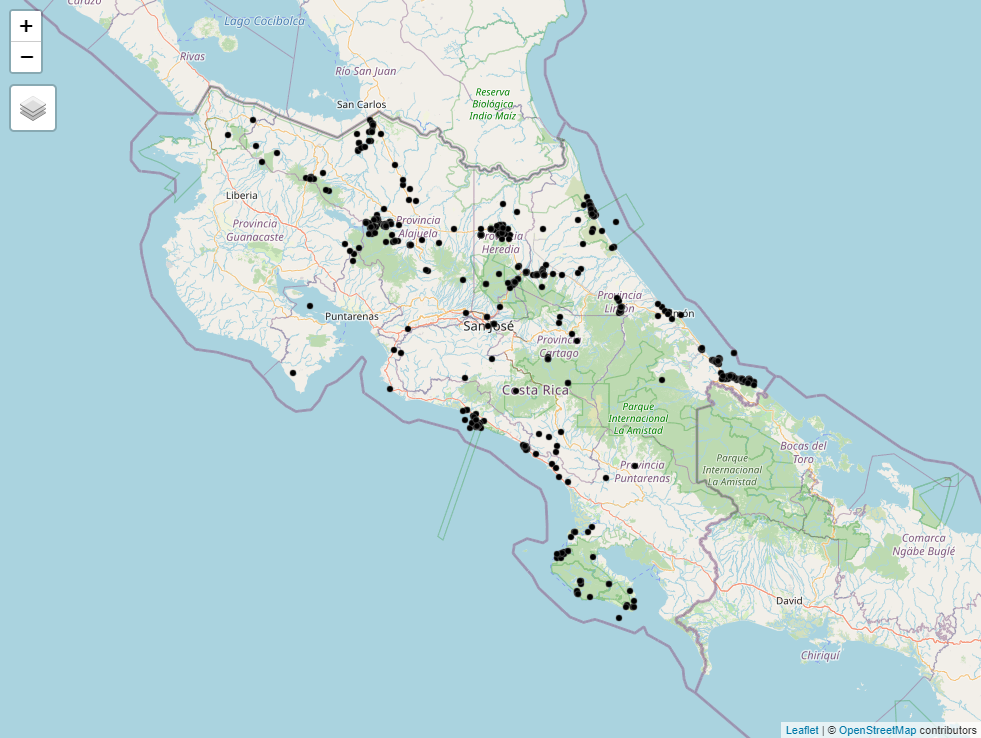
\includegraphics[width=.7\textwidth]{tmapview}
  \caption{Snapshot of the interactive map depicting sloth locations in Costa Rica. The map shows some areas with no sloths and other areas with sloth aggregations.
}
  \label{fig:tmapview}
\end{figure}



The map created is shown in Figure \ref{fig:tmapview}. The map shows an inhomogeneous pattern of sloths with concentrations in several locations of Costa Rica.
We will use a log-Gaussian Cox point process model to predict the intensity of the process that generates the sloth locations and assess the potential effect of climatic variables on the occurrence pattern.

\section{Spatial climatic covariates}

In the model, we include a spatial explanatory variable that can potentially affect sloth occurrence.
Specifically, we include a variable that denotes annual minimum temperature observed in the study region.
This variable can be obtained using the \pkg{raster} package \citep{Rraster} from the WorldClim database (\url{http://www.worldclim.org/bioclim}).
We use the \code{getData()} function of the \pkg{raster} package by specifying the name of the database (\code{"worldclim"}),
the variable name (\code{"tmin"}), and a resolution of 10 minutes of a degree (\code{"10"}).
\code{getData()} returns a \code{RasterStack} with minimum temperature observations with degree Celsius x 10 units for each month.
We average the values of the \code{RasterStack} and compute a raster that represents annual average minimum temperature.


\begin{example}
library(raster)
rmonth <- getData(name = "worldclim", var = "tmin", res = 10)
rcov <- mean(rmonth)
\end{example}



\section{Implementing and fitting the spatial point process model}

\subsection{Log-Gaussian Cox process model}


We assume that the spatial point pattern of sloth locations in Costa Rica, $\{x_i: i=1, \ldots, n\}$, has been generated as a realization of a  log-Gaussian Cox process with intensity given by $\Lambda(s)= exp(\eta(s))$.
This model can be easily fitted by approximating it by a latent Gaussian model by means of a gridding approach \citep{illianetal12}.
First, we discretize the study region into a grid with $n_1 \times n_2 = N$ cells $\{s_{ij}\}$, $i=1,\ldots,n_1$, $j=1,\ldots,n_2$.
In the log-Gaussian Cox process, the mean number of events in cell $s_{ij}$ is given by the integral of the intensity over the cell,
$\Lambda_{ij}=\int_{s_{ij}} exp(\eta(s))ds$, and
this integral can be approximated by
$\Lambda_{ij} \approx |s_{ij}| exp(\eta_{ij})$,
where $|s_{ij}|$ is the area of the cell $s_{ij}$.
Then, conditional on the latent field $\eta_{ij}$,
the observed number of locations in grid cell $s_{ij}$, 
$y_{ij}$, are independent and Poisson distributed as follows,
$$y_{ij}|\eta_{ij} \sim Poisson(|s_{ij}| exp(\eta_{ij})).$$
In our example, we model the log-intensity of the Poisson process as
$$\eta_{ij} = \beta_0 + \beta_1 \times cov(s_{ij}) + f_s(s_{ij}) + f_u(s_{ij}).$$
Here, $\beta_0$ is the intercept,
$cov(s_{ij})$ is the covariate value at $s_{ij}$, and
$\beta_1$ is the coefficient of $cov(s_{ij})$.
\code{f\_s()} is a spatially structured random effect reflecting unexplained variability that can be specified as a second-order two-dimensional CAR-model on a regular lattice.
\code{f\_u()} is an unstructured random effect reflecting independent variability in cell $s_{ij}$.


\subsection{Computational grid}

In order to fit the model, we create a regular grid that covers the region of Costa Rica.
First, we obtain a map of Costa Rica using the \code{ne\_countries()} function of the \CRANpkg{rnaturalearth} package \citep{Rrnaturalearth}. In the function we set \code{type = "countries"}, \code{country = "Costa Rica"} and \code{scale = "medium"} (\code{scale} denotes the scale of map to return and possible options are small, medium and large).

\begin{example}
library(rnaturalearth)
map <- ne_countries(type = "countries", country = "Costa Rica", scale = "medium")
\end{example}

Then, we create a raster that covers Costa Rica using \code{raster()} where we provide the map of Costa Rica and set \code{resolution = 0.1} to create cells with size of 0.1 decimal degrees.
This creates a raster with 31 $\times$ 33 = 1023 cells, each having an area equal to $0.1^2$ decimal degrees$^2$ (or 11.132 Km$^2$ at the equator).

\begin{example}
resolution <- 0.1
r <- raster(map, resolution = resolution)
(nrow <- nrow(r))
## [1] 31
(ncol <- ncol(r))
## [1] 33
nrow*ncol
## [1] 1023
\end{example}

We initially set to 0 the values of all the raster cells by using \code{r[] <- 0}.
Then, we use \code{cellFromXY()} to obtain the number of sloths in each of the cells, and assign these counts to each of the cells of the raster.

\begin{example}
r[] <- 0
tab <- table(cellFromXY(r, dpts))
r[as.numeric(names(tab))] <- tab
\end{example}

Finally, we convert the raster \code{r} to a \code{SpatialPolygonsDataFrame} object called \code{grid} using \code{rasterToPolygons()}.
This grid will be used to fit the model with the \pkg{R-INLA} package.

\begin{example}
grid <- rasterToPolygons(r)
\end{example}



\subsection{Data}

Now, we add to \code{grid} the data needed for modeling.
Since the spatial model that will be used in \pkg{R-INLA} assumes data are sorted by columns, we first transpose \code{grid}.
Then, we add variables \code{id} with the id of the cells, \code{Y} with the number of sloths, and \code{cellarea} with the cell areas.

\begin{example}
grid <- grid[as.vector(t(matrix(1:nrow(grid), nrow = ncol, ncol = nrow))), ]

grid$id <- 1:nrow(grid)
grid$Y <- grid$layer
grid$cellarea <- resolution*resolution
\end{example}


We also add a variable \code{cov} with the value of the minimum temperature covariate in each of the cells obtained with the \code{extract()} function of \pkg{raster}.

\begin{example}
grid$cov <- extract(rcov, coordinates(grid))
\end{example}

Finally, we delete the cells of \code{grid} that lie outside Costa Rica.
First, we use \code{raster::intersect()} to know which cells lie within the map, and then subset these cells in the \code{grid} object.

\begin{example}
gridmap <- raster::intersect(grid, map)
grid <- grid[grid$id %in% gridmap$id, ]
\end{example}

A summary of the data can be seen as follows,

\begin{example}
summary(grid)

## Object of class SpatialPolygonsDataFrame
## Coordinates:
##          min       max
## x -85.908008 -82.60801
## y   8.089453  11.18945
## Is projected: FALSE 
## proj4string :
## [+proj=longlat +datum=WGS84 +no_defs +ellps=WGS84 +towgs84=0,0,0]
## Data attributes:
##      layer             id               Y            cellarea         cov       
##  Min.   : 0.00   Min.   :   3.0   Min.   : 0.00   Min.   :0.01   Min.   : 78.0  
##  1st Qu.: 0.00   1st Qu.: 291.5   1st Qu.: 0.00   1st Qu.:0.01   1st Qu.:176.7  
##  Median : 0.00   Median : 566.0   Median : 0.00   Median :0.01   Median :202.4  
##  Mean   : 1.38   Mean   : 533.1   Mean   : 1.38   Mean   :0.01   Mean   :189.0  
##  3rd Qu.: 0.00   3rd Qu.: 762.5   3rd Qu.: 0.00   3rd Qu.:0.01   3rd Qu.:211.2  
##  Max.   :95.00   Max.   :1009.0   Max.   :95.00   Max.   :0.01   Max.   :223.2  
##                                                                  NA's   :2      
\end{example}

We observe that the minimum temperature covariate has 2 missing values. We decide to impute these missing values with a simple approach where we set these values equal to the values of the cells next to them.

\begin{example}
indNA <- which(is.na(grid$cov))
indNA

## [1]   6 220

grid$cov[indNA] <- grid$cov[indNA+1]
\end{example}

We use \pkg{tmap} to create maps of the number of sloths (\code{Y}) and the covariate values (\code{cov}).
In the maps, we plot the border of \code{grid} that we obtain with the \code{gUnaryUnion()} function of the \CRANpkg{rgeos} package \citep{Rrgeos}.

\begin{example}
library(rgeos)
gridborder <- gUnaryUnion(grid)
\end{example}

We use \code{tm\_facets(ncol = 2)} to plot maps in the same row and two columns, and \code{tm\_legend()} to put the legends in the left-bottom corner of the plots (Figure \ref{fig:tmapYcov}).

\begin{example}
tmap_mode("plot")
tm_shape(grid) +
  tm_polygons(col = c("Y", "cov"), border.col = "transparent") +
  tm_shape(gridborder) + tm_borders() +
  tm_facets(ncol = 2) + tm_legend(legend.position = c("left", "bottom"))
\end{example}



\begin{figure}[htbp]
  \centering
  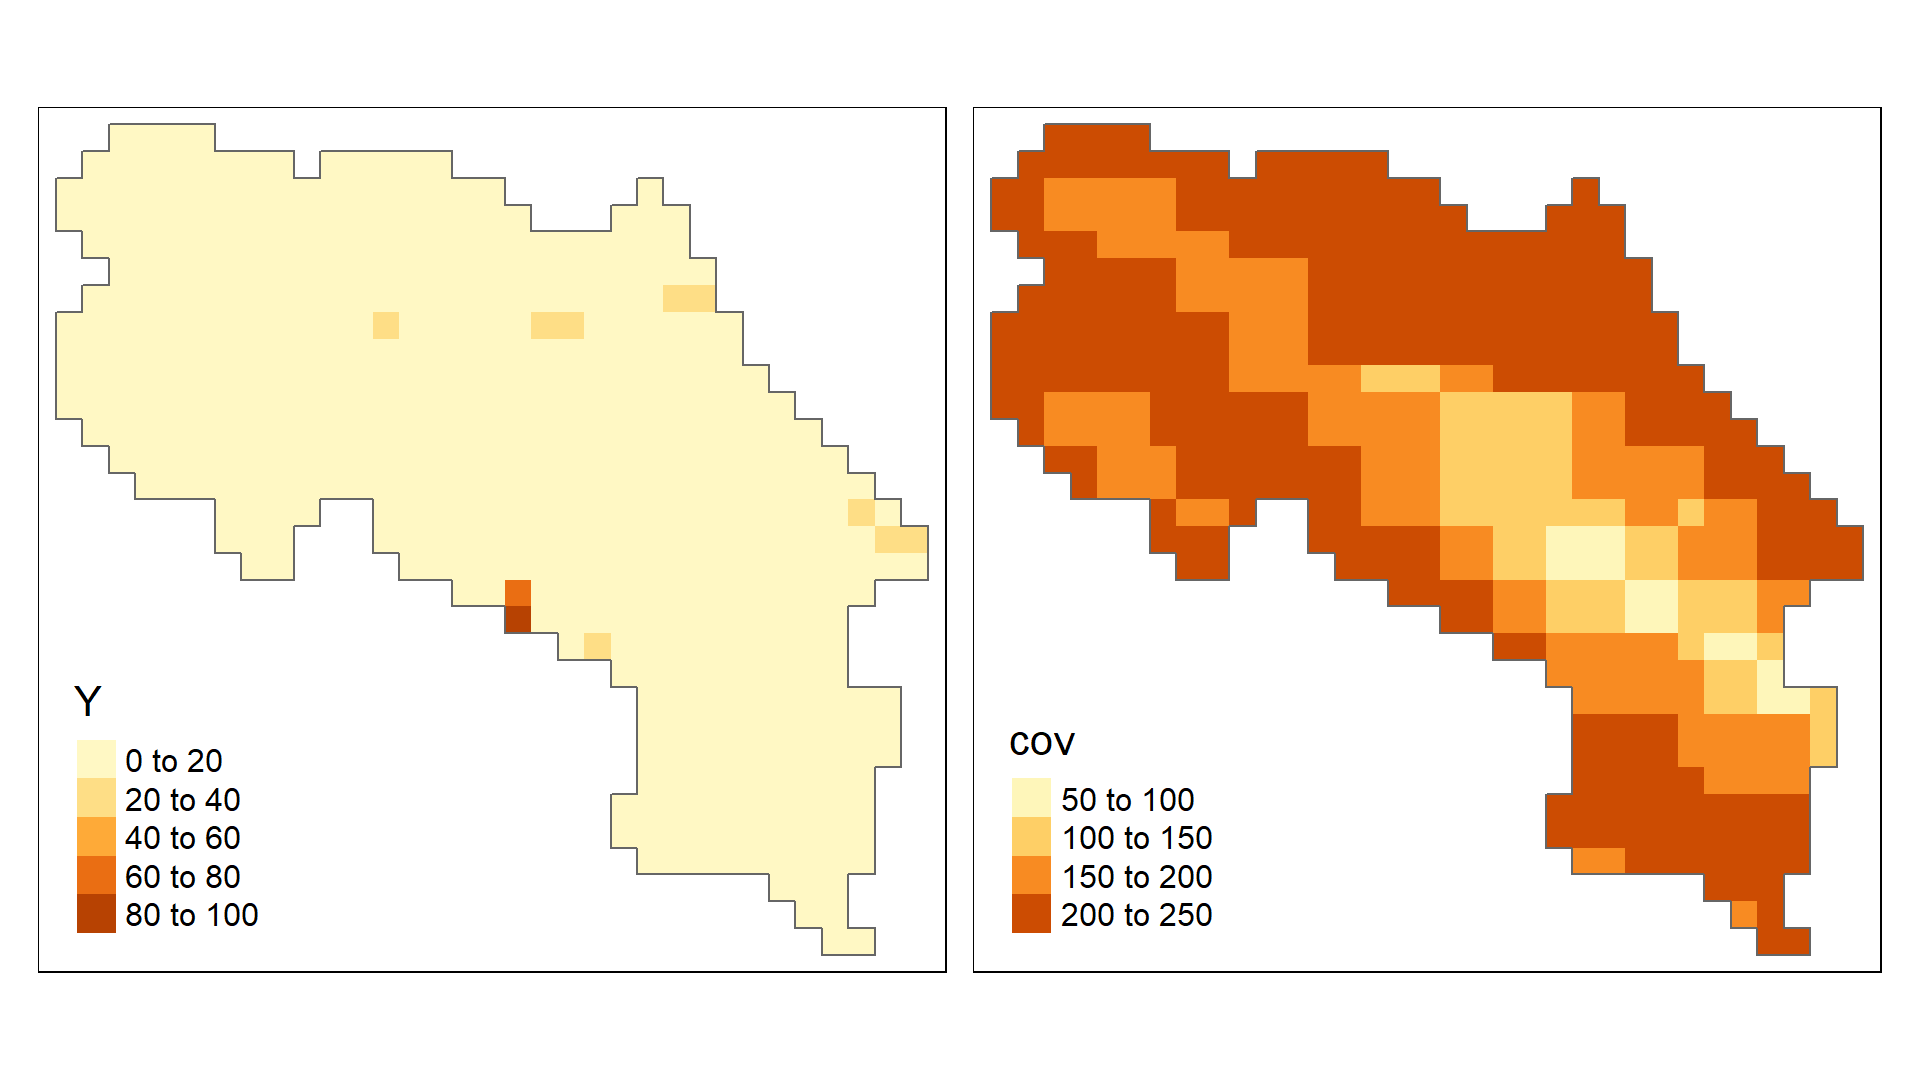
\includegraphics[width=.8\textwidth]{tmapYcov}
  \caption{Maps with the number of sloths (left) and minimum temperature values (right) in Costa Rica. The intensity of sloths occurrence is modeled using minimum temperature as a covariate.
}
  \label{fig:tmapYcov}
\end{figure}



\subsection{Fitting the model using \pkg{R-INLA}}



We fit the log-Gaussian Cox process model to the sloths data using the \pkg{R-INLA} package. This package implements the integrated nested Laplace approximation (INLA) approach that permits to perform approximate Bayesian inference in latent Gaussian models \citep{rueetal09, moraga19}.
\pkg{R-INLA} is not on CRAN because it uses some external C libraries that make difficult to build the binaries. 
Therefore, when installing the package, we need to specify the URL of the R-INLA repository.
We also need to add the \url{https://cloud.r-project.org} repository to enable the installation of CRAN dependencies as follows,

\begin{example}
install.packages("INLA", repos = c("https://inla.r-inla-download.org/R/stable",
                                   "https://cloud.r-project.org"), dep = TRUE)
\end{example}


Note that the \pkg{R-INLA} package is large and its installation may take a few minutes.
Moreover, \pkg{R-INLA} suggests the \BIOpkg{graph} and \BIOpkg{Rgraphviz} packages which are part of the Bioconductor project. These packages have to be installed by using their tools, for example, by using\\  
\code{BiocManager::install(c("graph", "Rgraphviz"), dep = TRUE))}.


To fit the model in INLA we need to specify a formula with the linear predictor, and then call the \code{inla()} function providing the formula, the family, the data, and other options.
The formula is written by writing the outcome variable,
then the $\sim$ symbol, and then the fixed and random effects separated by \code{+} symbols.
By default, the formula includes an intercept.
The outcome variable is \code{Y} (the number of occurrences in each cell) and the covariate is \code{cov}.
The random effects are specified with the \code{f()} function where the first argument is an index vector specifying which elements of the random effect apply to each observation, and the other arguments are the model name and other options.
In the formula, different random effects need to have different indices vectors.
We use \code{grid\$id} for the spatially structured effect,
and create an index vector \code{grid\$id2} with the same values as \code{grid\$id}
for the unstructured random effect.
The spatially structured random effect is specified with the index vector \code{id}, the model name that corresponds to ICAR(2) (\code{"rw2d"}), and the number of rows (\code{nrow}) and columns (\code{ncol}) of the regular lattice. 
The unstructured random effect is specified with the index vector \code{id2} and the model name \code{"iid"}.

\begin{example}
library(INLA)

grid$id2 <- grid$id

formula <- Y ~ 1 + cov +
  f(id, model="rw2d", nrow = nrow, ncol = ncol) +
  f(id2, model="iid")
\end{example}

Finally, we call \code{inla()} where we provide the formula, the family (\code{"poisson"}) and the data (\code{grid@data}). We write \code{E = cellarea} to denote that the expected values in each of the cells are in variable \code{cellarea} of the data.
We also write \code{control.predictor = list(compute = TRUE)} to compute the marginal densities for the linear predictor.



\begin{example}
res <- inla(formula, family = "poisson", data = grid@data,
            E = cellarea, control.predictor = list(compute = TRUE))
\end{example}


\subsection{Results}

The execution of \code{inla()} returns an object \code{res} that contains information about the fitted model including the posterior marginals of the parameters and the intensity values of the spatial process.
We can see a summary of the results as follows,

\begin{example}
summary(res)

## Fixed effects:
##               mean    sd 0.025quant 0.5quant 0.975quant   mode kld
## (Intercept) -1.904 2.426     -6.832   -1.852      2.734 -1.754   0
## cov          0.016 0.009     -0.002    0.016      0.035  0.016   0
## 
## Random effects:
##   Name	  Model
##     id Random walk 2D
##    id2 IID model
## 
## Model hyperparameters:
##                    mean    sd 0.025quant 0.5quant 0.975quant  mode
## Precision for id  0.474 0.250      0.158    0.420       1.11 0.328
## Precision for id2 0.287 0.055      0.193    0.282       0.41 0.272
## 
## Expected number of effective parameters(stdev): 196.11(7.06)
## Number of equivalent replicates : 2.61 
## 
## Marginal log-Likelihood:  -1620.60 
## Posterior marginals for the linear predictor and the fitted values are computed
\end{example}


The intercept $\hat \beta_0 = -1.904$ with 95\% credible interval $(-6.832, 2.734)$,
the minimum temperature covariate has a positive
effect on the intensity of the process with a posterior mean $\hat \beta_1 = 0.016$ and 95\% credible interval $(-0.002, 0.035)$.
We can plot the posterior distribution of the coefficient of the covariate $\hat \beta_1$ with \pkg{ggplot2} (Figure \ref{fig:ggplot2cov}).
First, we calculate a smoothing of the marginal distribution of the coefficient with \code{inla.smarginal()} and then call \code{ggplot()} specifying the data frame with the marginal values.

\begin{example}
library(ggplot2)
marginal <- inla.smarginal(res$marginals.fixed$cov)
marginal <- data.frame(marginal)
ggplot(marginal, aes(x = x, y = y)) + geom_line() +
  labs(x = expression(beta[1]), y = "Density") +
  geom_vline(xintercept = 0, col = "black") + theme_bw()
\end{example}



\begin{figure}[htbp]
  \centering
  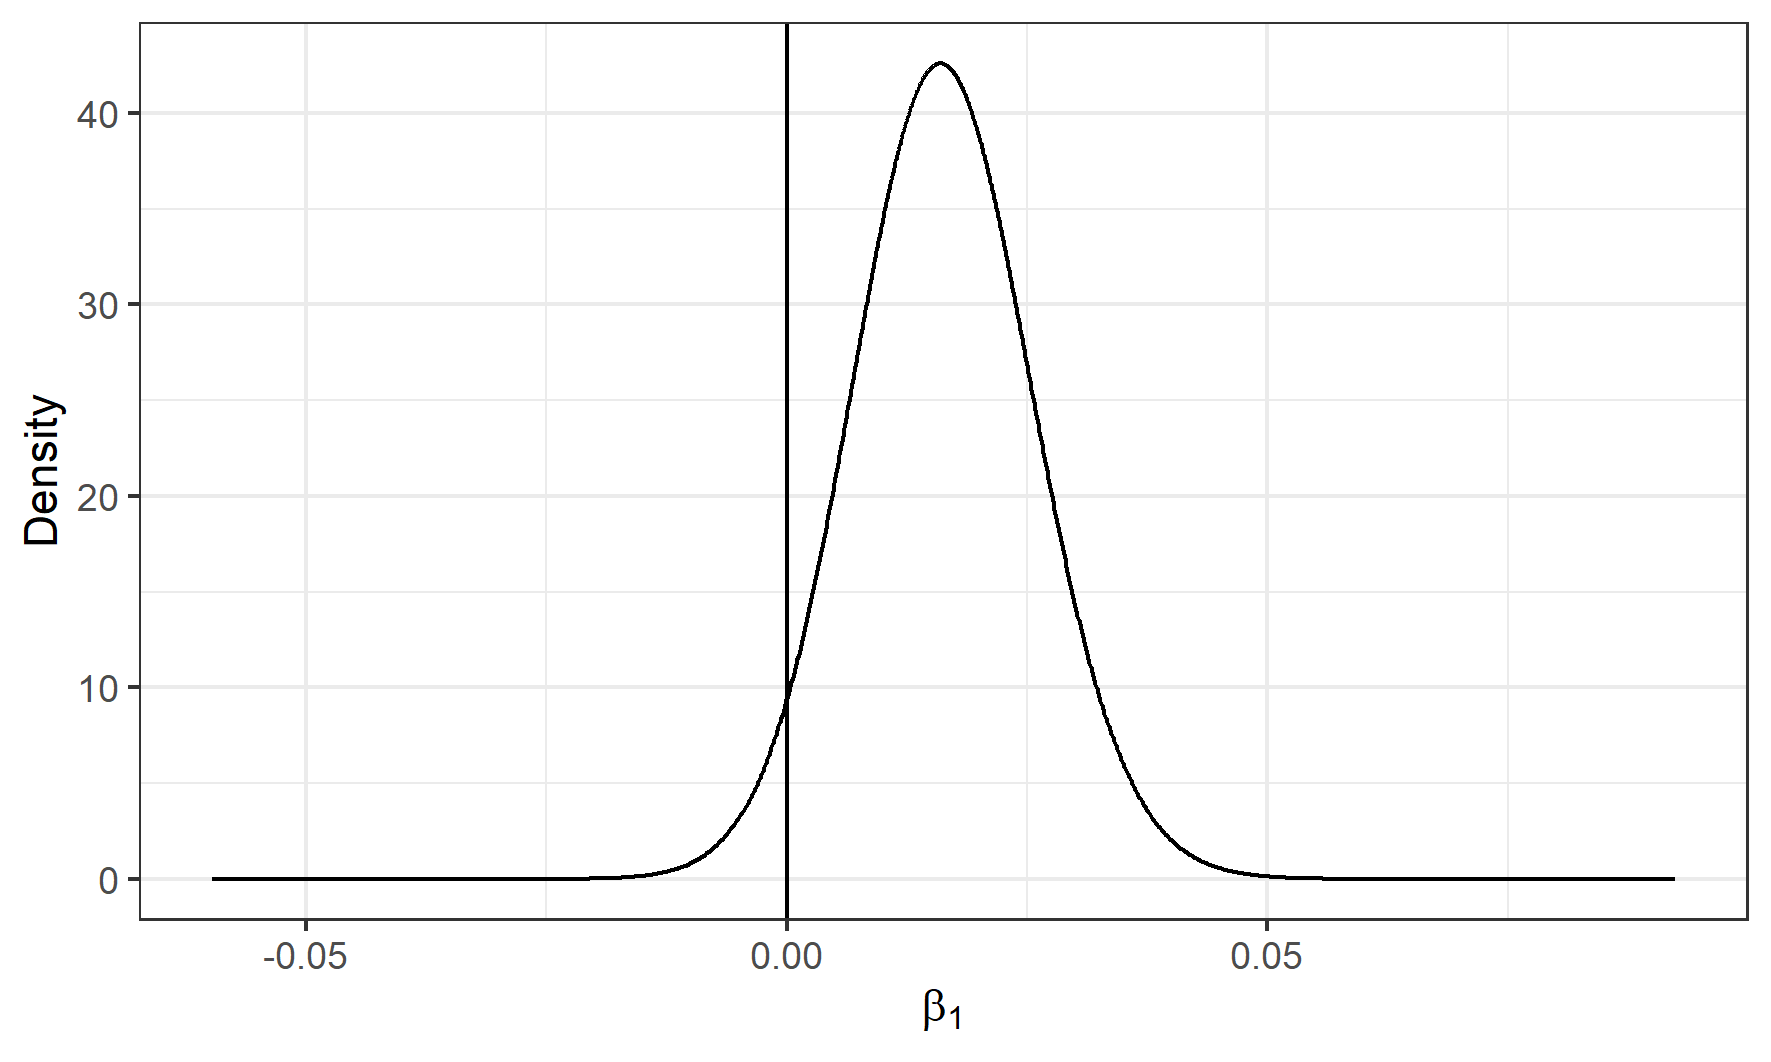
\includegraphics[width=.8\textwidth]{ggplot2cov2}
  \caption{Posterior distribution of the coefficient of covariate minimum temperature and a vertical line at 0. The posterior mean is positive and the 95\% credible interval includes 0.
}
  \label{fig:ggplot2cov}
\end{figure}



The estimated spatially structured effect is in
\code{res\$summary.random\$id}. This object contains 1023 elements that correspond to the number of cells in the regular lattice. We can add to the \code{grid} object the posterior mean of the spatial effect corresponding to each of the cells in Costa Rica as follows,


\begin{example}
grid$respa <- res$summary.random$id[grid$id, "mean"]
\end{example}



We can also obtain the posterior mean of the unstructured random effect as follows,
\begin{example}
grid$reiid <- res$summary.random$id2[, "mean"]
\end{example}

Then we can create maps of the random effects with \pkg{tmap}.

\begin{example}
tm_shape(grid) +
  tm_polygons(col = c("respa", "reiid"), style = "cont", border.col = "transparent")  +
  tm_shape(gridborder) + tm_borders() +
  tm_facets(ncol = 2) + tm_legend(legend.position = c("left", "bottom"))
\end{example}


\begin{figure}[htbp]
  \centering
  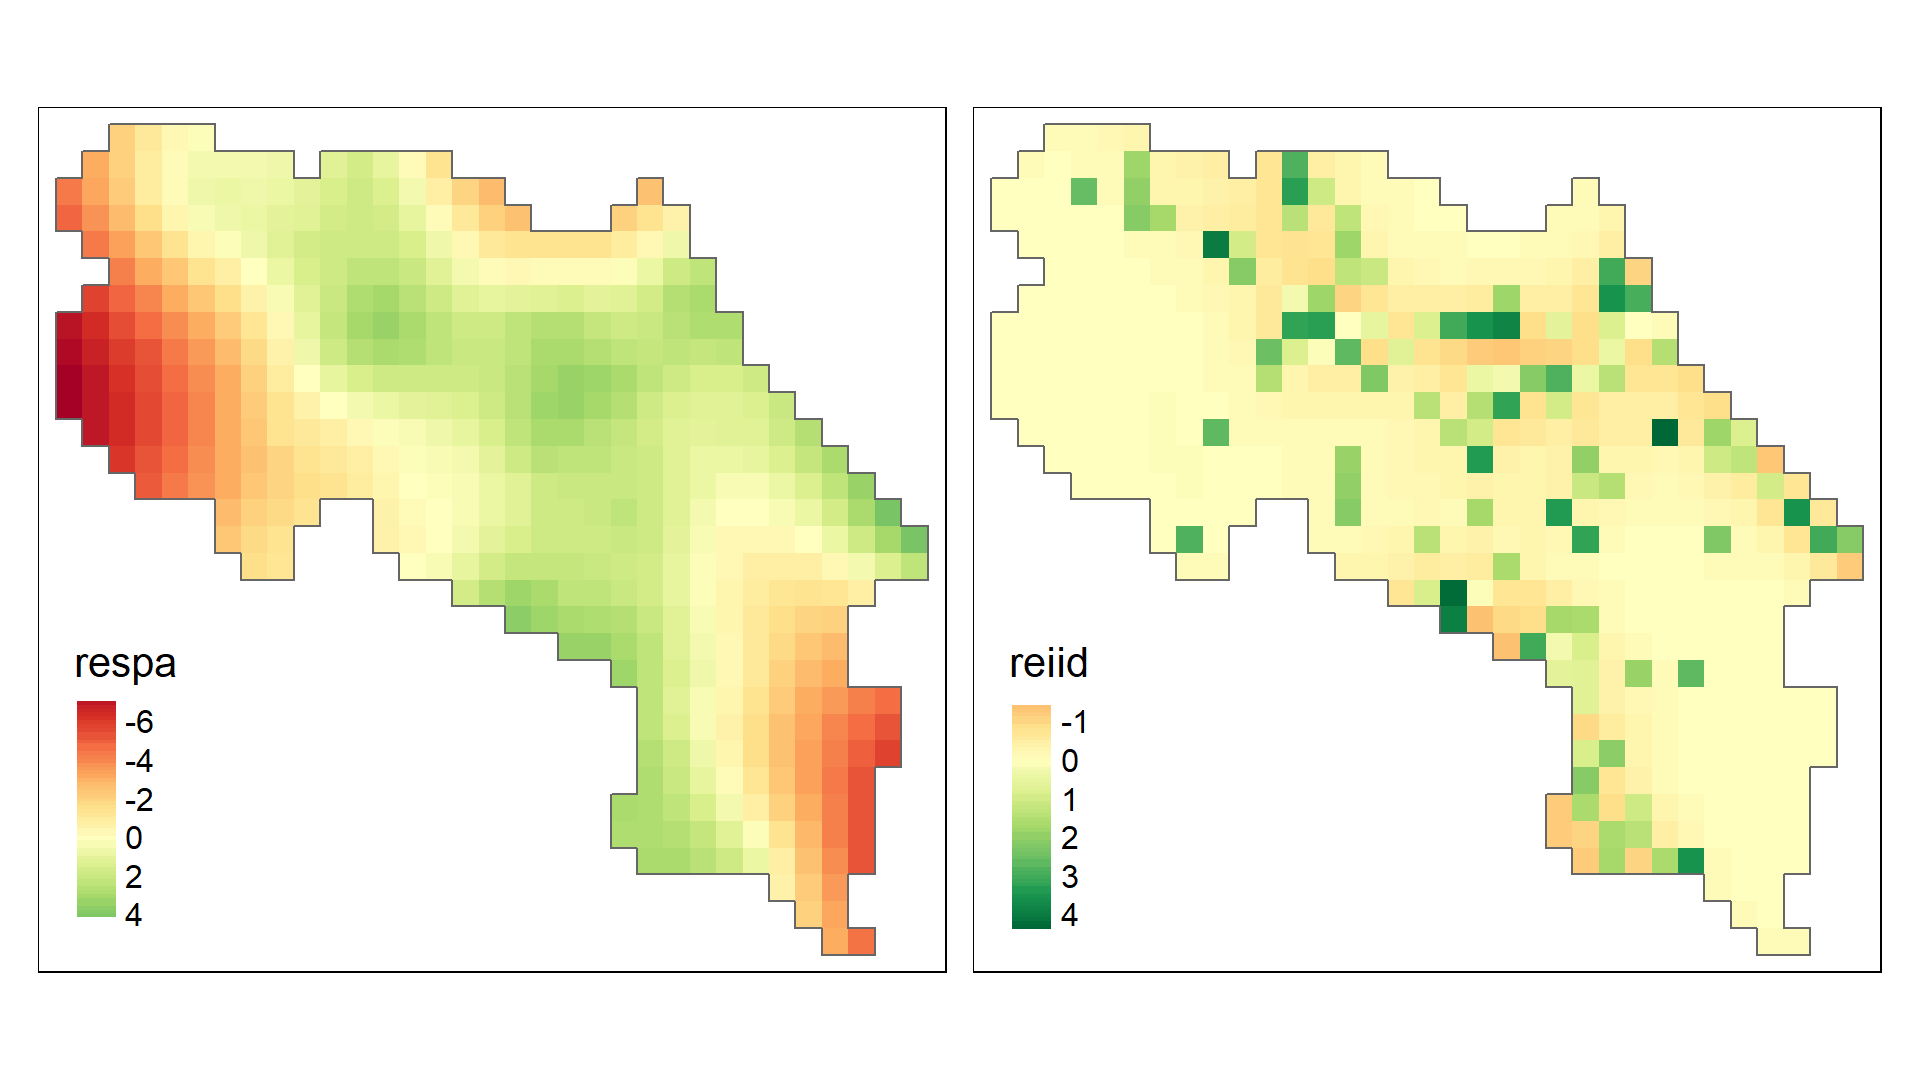
\includegraphics[width=.8\textwidth]{tmaprandomeffects}
  \caption{Maps with the values of the spatially structured (left) and unstructured (right) random effects. Maps show there is spatially structured and unstructured residual variation.
}
  \label{fig:tmaprandomeffects}
\end{figure}

Figure \ref{fig:tmaprandomeffects} shows the maps of the spatially structured and unstructured random effects.
We observe a non-constant pattern of the spatially structured random effect suggesting that the intensity of the process that generates the sloth locations may be affected by other spatial factors that have not been considered in the model.
Morevoer, the unstructured random effect shows several locations with high values that modify the intensity of the process in individual cells independently from the rest.

The mean and quantiles of the predicted intensity (mean number of events per unit area) in each of the grid cells are in \code{res\$summary.fitted.values}. In the object \code{grid}, we add a variable \code{NE} with the mean number of events of each cell by assigning the predicted intensity multiplied by the cell areas. We also add variables \code{LL} and \code{UL} with the lower and upper limits of 95\% credible intervals for the number of events by assigning quantiles 0.025 and 0.975 multiplied by the cell areas.

\begin{example}
cellarea <- resolution*resolution
grid$NE <- res$summary.fitted.values[, "mean"] * cellarea
grid$LL <- res$summary.fitted.values[, "0.025quant"] * cellarea
grid$UL <- res$summary.fitted.values[, "0.975quant"] * cellarea
\end{example}

We use \pkg{tmap} to create maps with the mean and lower and upper limits of 95\% credible intervals for the number of sloths in each of the cells.
We plot the three maps with a common legend that has breaks from 0 to the maximum number of cases in \code{grid\$UL}.

\begin{example}
tm_shape(grid) +
  tm_polygons(col = c("NE", "LL", "UL"),
              style = 'fixed', border.col = "transparent",
              breaks = c(0, 10, 50, 100, ceiling(max(grid$UL)))) +
  tm_shape(gridborder) + tm_borders() +
  tm_facets(ncol = 3) + tm_legend(legend.position = c("left", "bottom")) 
\end{example}


\begin{figure}[htbp]
  \centering
  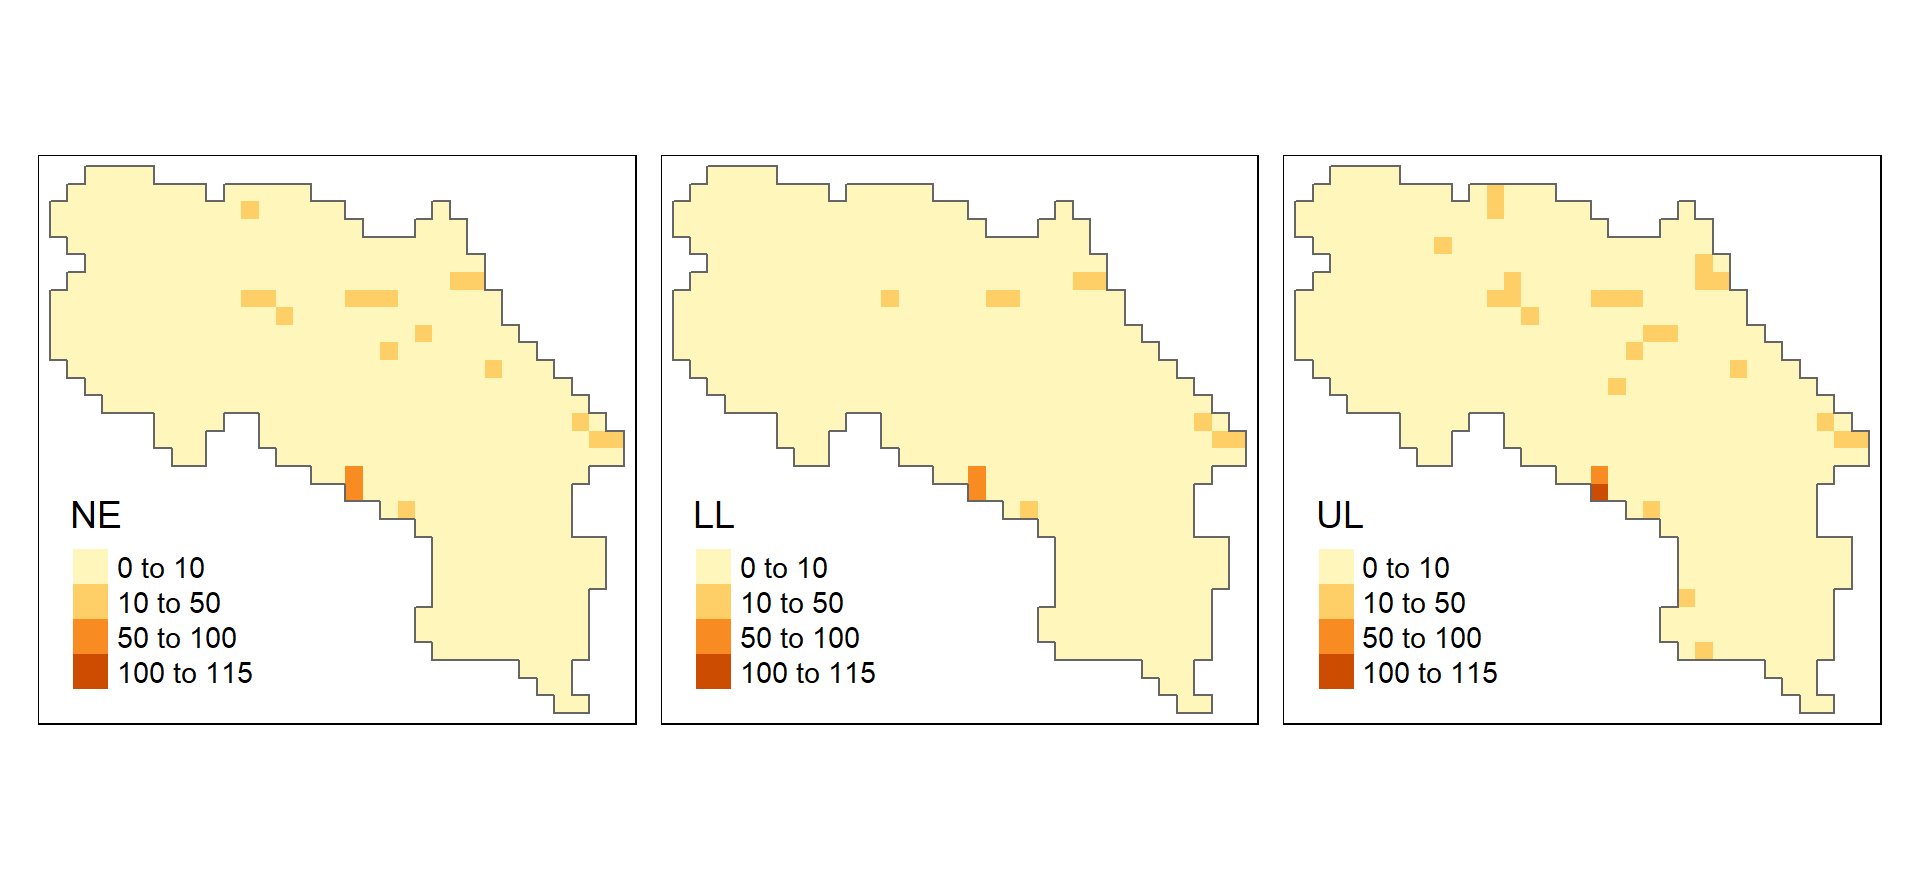
\includegraphics[width=1\textwidth]{tmapintensity}
  \caption{Maps with the predicted mean number of sloths (left), and lower (center) and upper (right) limits of 95\% credible intervals. Maps show low intensity of sloth occurrence overall, and some specific locations with high intensity.}
  \label{fig:tmapintensity}
\end{figure}


Maps created are shown in Figure \ref{fig:tmapintensity}.
We observe that overall, the intensity of sloth occurrence is low, with less than 10 sloths in each of the cells. We also see there are some locations of high sloth intensity in the west and east coasts and the north of Costa Rica. The maps with the lower and upper limits of 95\% credible intervals denote the uncertainty of these predictions.
The maps created inform about the spatial patterns in the period where the data were collected. In addition, maps of the sloth numbers over time can also be produced using spatio-temporal point process models and this would help understand spatio-temporal patterns.
The modeling results can be useful for decision-makers to identify areas of interest for conservation management strategies.



\section{Summary}

Species distribution models are widely used in ecology for conservation management of species and their environments. In this paper, we have described how to develop and fit a log-Gaussian Cox process model
using the \pkg{R-INLA} package
to predict the intensity of species occurrence, and assess the effect of spatial explanatory variables.
We have illustrated the modeling approach using sloth occurrence data in Costa Rica retrieved from the Global Biodiversity Information Facility database (GBIF) using \pkg{spocc}, and a spatial climatic variable obtained with \pkg{raster}.
We have also shown how to examine and interpret the results
including the estimates of the parameters and the intensity of the process, and how to create maps of variables of interest using \pkg{tmap}.


Statistical packages such as Stan \citep{stan} or JAGS \citep{jags} could have been used instead of \pkg{R-INLA} to fit our data.
However, these packages use Markov chain Monte Carlo (MCMC) algorithms and may be high computationally demanding and become infeasable in large spatial data problems. In contrast, INLA produces faster inferences which allows us to fit large spatial datasets and explore alternative models.

The objective of this paper is to illustrate how to analyze species occurrence data using spatial point process models and cutting-edge statistical techniques in R.
Therefore, we have ignored the data collection methods and have assumed that the spatial pattern analyzed is a realization of the true underlying process that generates the data.
In real investigations, however, it is important to understand the sampling mechanisms, and assess potential biases in the data such as overrepresentation of certain areas that can invalidate inferences.
Ideally, we would analyze data that have been obtained using well-defined sampling schemes. Alternatively, we would need to develop models that adjust for biases in the data to produce meaningful results \citep{giraudetal15, dorazio14, fithianetal15}.
Moreover, expert knowledge is crucial to be able to develop appropriate models that include important predictive covariates and random effects that account for different types of variability.

To conclude, this paper provides an accessible illustration of spatial point process models and computational approaches that can help non-statisticians analyze spatial point patterns using R.
We have shown how to use these approaches in the context of species distribution modeling, but they are also useful to analyze spatial data that arise in many other fields such as epidemiology and the environment.


\bibliography{moraga}

\address{Paula Moraga\\
Computer, Electrical and Mathematical Sciences and Engineering Division\\ King Abdullah University of Science and Technology (KAUST)\\
Thuwal, 23955-6900\\
Saudi Arabia\\
ORCiD: 0000-0001-5266-0201\\
Webpage: \url{http://www.paulamoraga.com/}\\
\email{paula.moraga@kaust.edu.sa}}


